%----------------------------------------------------------------------------
\chapter{Model-based testing}
\label{cha:modelbasedtesting}
%----------------------------------------------------------------------------

The idea of model-based testing originates from the 70's, and now it has an extensive literature, terminology and a commonly accepted taxonomy \cite{taxonomy}. This section introduces the concept of this variant of software testing through a concrete process (Figure~\ref{fig:mbtprocess}).

\begin{figure}[htp]
\centering
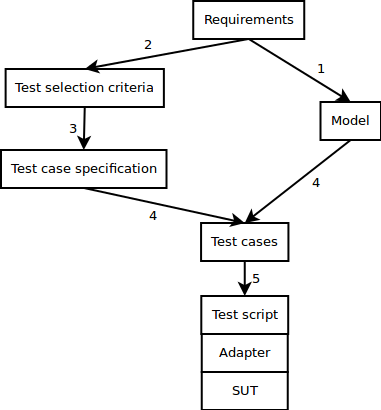
\includegraphics[scale=0.6]{figures/mbt_process.png}
\caption{Model-based testing process}
\label{fig:mbtprocess}
\end{figure}

\begin{enumerate}
    \item From informal requirements or created specifications a model can be built. The model is an abstract representation of the \textit{system under test (SUT)}. It uses encapsulation to information reduction, because it has to be more simple, than the original system to achieve an easier modifying, maintaining \cite{mbttestcasegeneration}. During a model-based software development it can be used for many other tasks too, as the model serves analysing, synthesising and documenting the SUT as well.
     \item Test selection criteria decide how the test cases are chosen, which point of view is important by testing. Further details are at the subsection~\ref{sub:taxonomy}.
     \item Criteria are transformed into test case specifications. These test case specifications are the formalised versions of the critera.
     \item After creating the model and the test case specifications set of test cases is generated from the model regarding all the specifications. One of the biggest challenges is to create the \textit{test cases}. A simple test case consists of a pair of input parameters and expected outputs. Finite set of test cases forms a \textit{test suite}. The difficulty comes from the need to satisfy the test case specifications and create a minimised set of test cases.
     \item A successfully generated test suite can be executed on the SUT. For the execution a \textit{test script} can be used, which executes the test cases.
     
     The generated test cases are strongly linked to the abstract test model, therefore an \textit{adaptor} component is needed, which is often part of the test script. The adaptor adapts the test inputs to the SUT. For example if the input of a method is an XML document containing an integer value, the adaptor has to transform the test case's test inputs to XML.
     
     The test script also contains usually a \textit{test oracle}, that checks the test output difference from the expected output.
\end{enumerate}

\section{Terminology}
\label{sec:terminology}

...

% section terminology (end)

\section{Taxonomy}
\label{sec:taxonomy}

Utting, Pretschner and Legeard investigated the currently available MBT solutions and defined (Figure~\ref{fig:mbttaxonomy}) a taxonomy which concentrates to three major properties of model-based testing. The three dimensions of their taxonomy are the modelling specification, test generation and test execution.

\begin{figure}[htp]
\centering
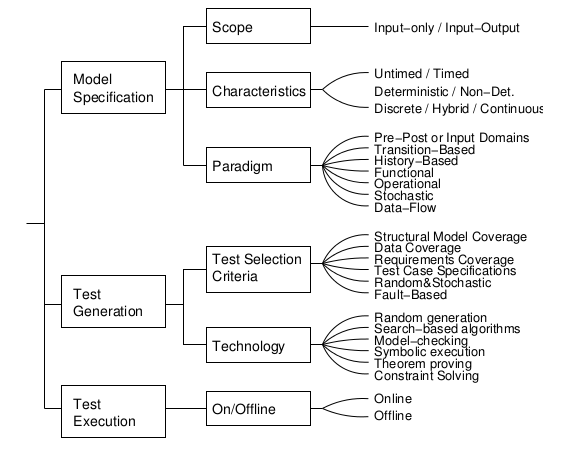
\includegraphics[scale=0.5]{figures/mbt_taxonomy.png}
\caption{Model-based testing taxonomy \cite{taxonomy}}
\label{fig:mbttaxonomy}
\end{figure}

\begin{description}
	\item[Model scope] The scope of the modelling is a binary decision. The model either specify \textit{just the test input} or \textit{the input-output pairs} for the SUT. The first case is less useful, because the test script can not check the SUT's output and that's why it is impossible to create an oracle that way.
	
	\item[Model characteristics] The SUT assigns the main characteristics of the model. It depends on the SUT's timing properties (\textit{timed} / \textit{untimed}), determinism (\textit{deterministic} / \textit{non-deterministic}) and dynamics (\textit{discrete} / \textit{continuous} / \textit{hybrid}).
	
	\item[Model paradigm] The third dimension is the paradigm that is used to describe the model. \textit{State-based notation} means, that set of variables defines the model, which represents the internal state of the system. By \textit{transition-based notation} the model focuses on the transition between the state of the system. Finite state machines are examples for this paradigm. \textit{History-based notations} model the allowable traces of its behaviour over time. By \textit{functional notation} collection of mathematical functions model the system. \textit{Operational notations} describe the model as a set of executable processes running parallel. \textit{Stochastic notations} describe the model by a probabilistic model, as it is rather suitable to model the environment than the SUT itself. The last paradigm is the \textit{data-flow notation}, where the main concept is the concentration to the data, rather than the control flow.
	
	\item[Test selection criteria] Test selection criteria control the test case generation. \textit{Structural model coverage criteria} aim to cover a part of the model, for example nodes and arcs of the transition-based model. The basic idea of \textit{data coverage criteria} is to split the data space to equivalence classes and choose values from them. \textit{Requirements based coverage criteria} are linked to the informal requirements of the SUT and it applies the coverage to the requirements. \textit{Ad-hoc test case specifications} guides by the test case specifications. \textit{Random and Stochastic criteria} are useful rather to model the environment and applicable to use with a stochastic model. \textit{Fault-based criteria} can be very efficient, because it concentrates to error finding in the SUT.
	
	\item[Test generation technology] One of the most important thing that defines the test case generation is the chosen technology. The easiest one to implement is the \textit{random generation}, more difficult are the \textit{search-based algorithms} where graph algorithms and other search algorithms are used to perform a walk on the model. \textit{Model checking} can also be used for test case generation, where the model checker searches for a counter-example, which becomes a test case. \textit{Symbolic execution} means analysing the software to determine what inputs cause each part of a program to execute. This method guided by test case specification to reach a goal, and test inputs become inputs which produce different outputs. \textit{Deductive theorem proving} is similar to model checking, but the model checker is replaced with a theorem prover. \textit{Constraint solving} is useful for selecting data values from complex data domains.
	
	\item[Test execution] The tests can run either \textit{online} or \textit{offline} on the SUT. During an online test, the test generator can respond to the SUT's actual output for example with an different test case sequence. By an offline test generation test cases are generated strictly before the execution.
	
	The testing can be started by an automatic execution or manually, that triggers the user directly.
\end{description}

% section taxonomy (end)

\section{Process}
\label{sec:process}

...

% section process (end)

% chapter modelbasedtesting (end)